\documentclass{article}

\author{Artur Amaral}
\title{EEL480 - Laboratório de Sistemas Digitais Relatório 01}


\usepackage[T1]{fontenc}
\usepackage{listings}
\usepackage[utf8]{inputenc}
\usepackage[portuguese]{babel}
\usepackage{hyphenat}
\hyphenation{mate-mática recu-perar}
\usepackage{graphicx}

\begin{document}

\maketitle

\section{Introdução}

\section{Desenvolvimento do projeto}
\begin{itemize}
    \item Duas entradas X e Y de 4 bits.
    \item Faixa de valores representada:
        \begin{itemize}
            \item  0 <= X, Y <= 15
            \item  -15 <= Z <= 15
        \end{itemize}
    \item Flags só possuem sentido explícito nas operações de adição e subtração.
\end{itemize}

\begin{center}
    \begin{tabular}{ c|c|c }

        \textbf{Seleção} & \textbf{Operação} & \textbf{Descrição} \\
    000 & RESET & Força zero\\
    001 & X MAIS Y & Adição\\
    010 & X MENOS Y & Subtração\\
    011 & X AND Y & And bit a bit\\
    100 & X OR Y & Or bit a bit\\
    101 & X XOR Y & Xor bit a bit\\
    110 & NOT X & Not bit a bit\\
    111 & PRESET & Força um\\


\end{tabular}
\end{center}

\begin{verbatim}
\end{verbatim}

\begin{center}
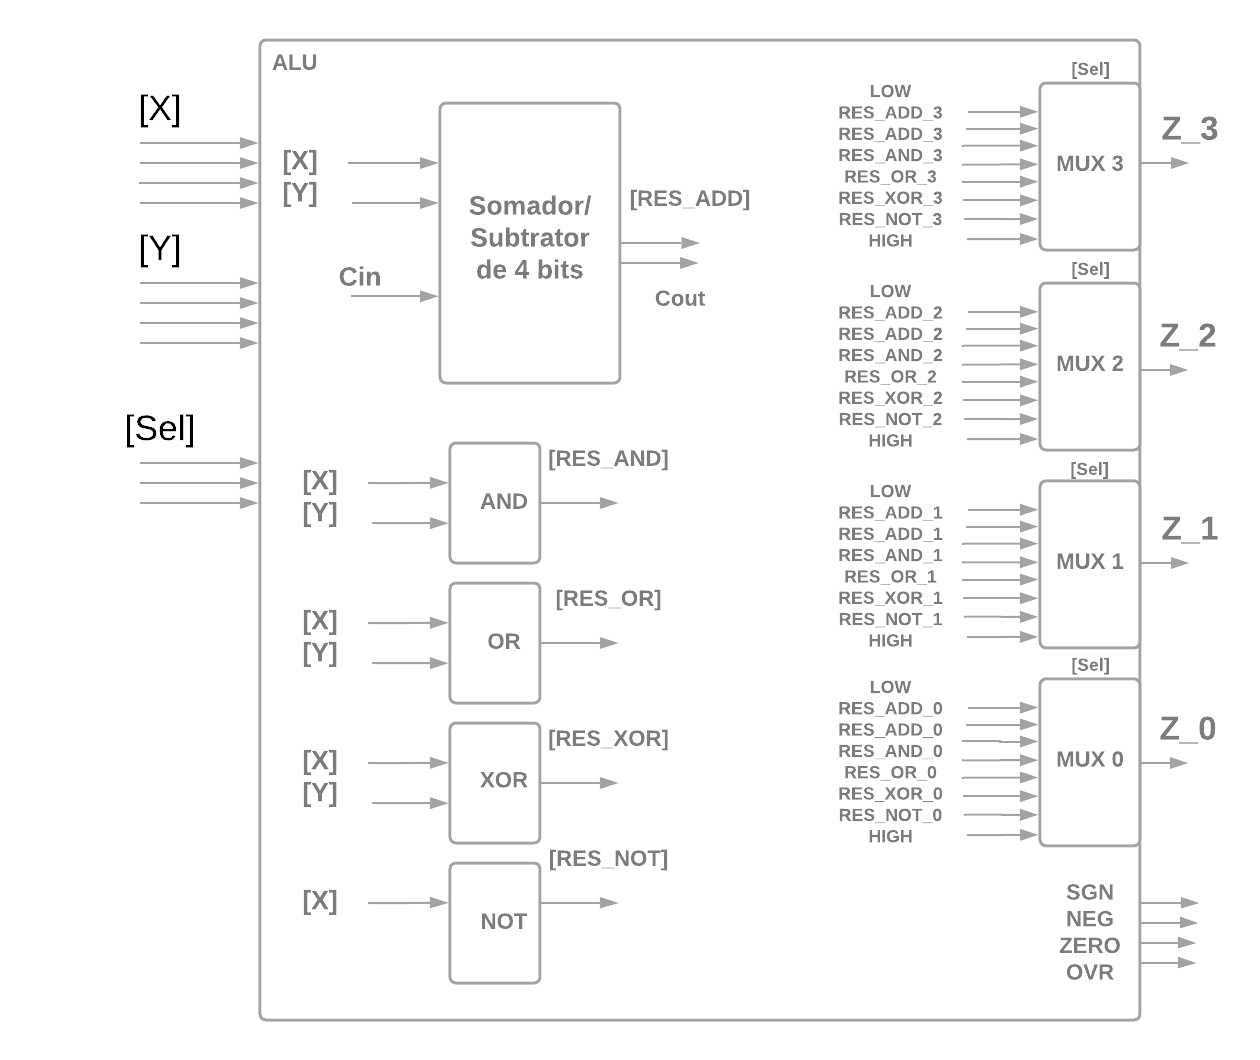
\includegraphics[width=\textwidth]{img/DB_ALU.png}
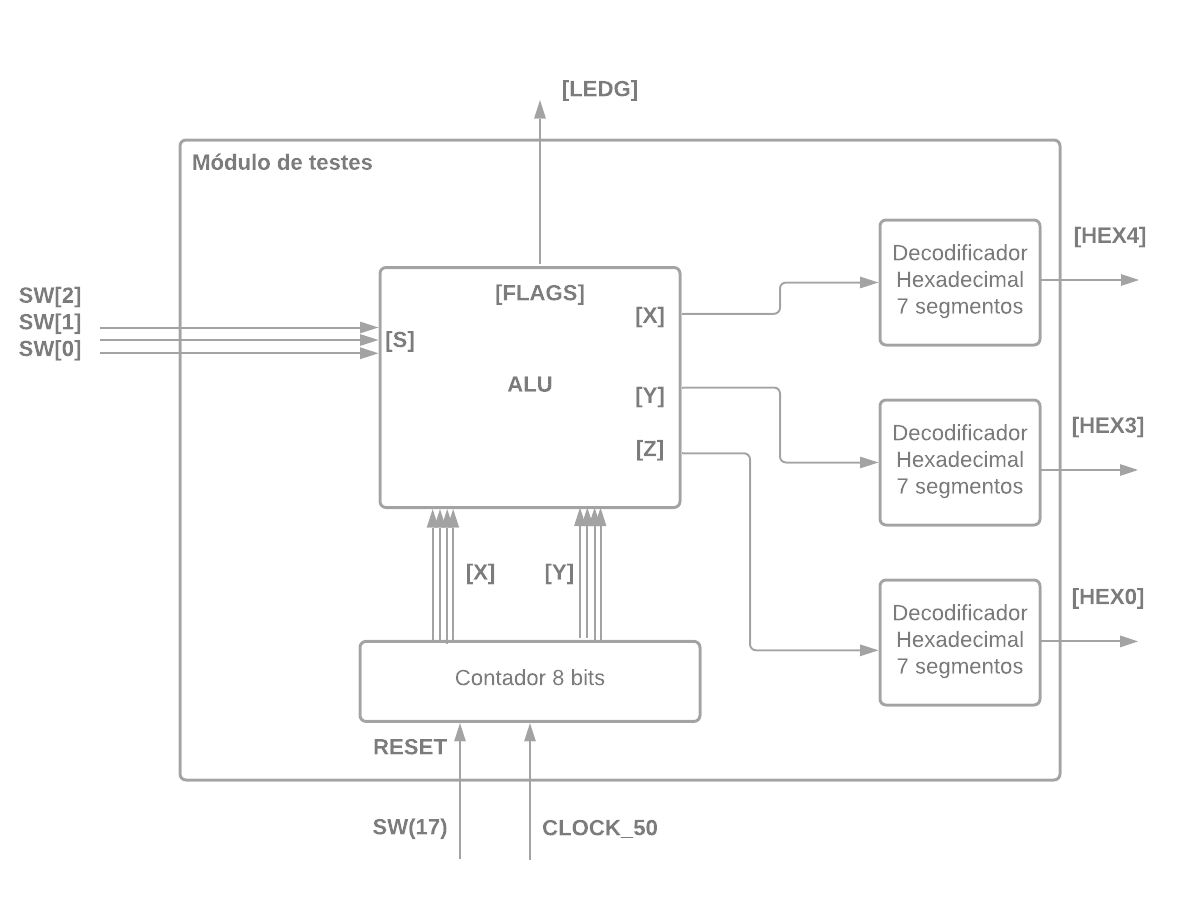
\includegraphics[width=\textwidth]{img/DB_Teste.png}
\end{center}

\textbf{Modularização em VHDL / Hierarquia dos arquivos}

\begin{verbatim}
ALU_testbench.vhd
|
|_counter_8bits.vhd
|_hex_to_display.vhd
|_ALU.vhd
   |
   |_fullAdder.vhd
   |_addSub4bits.vhd
   |_and4bits.vhd
   |_or4bits.vhd
   |_xor4bits.vhd
   |_not4bits.vhd
   |_mux_8_to_1.vhd

\end{verbatim}



\begin{center}

\textbf{Teste multiplexador}
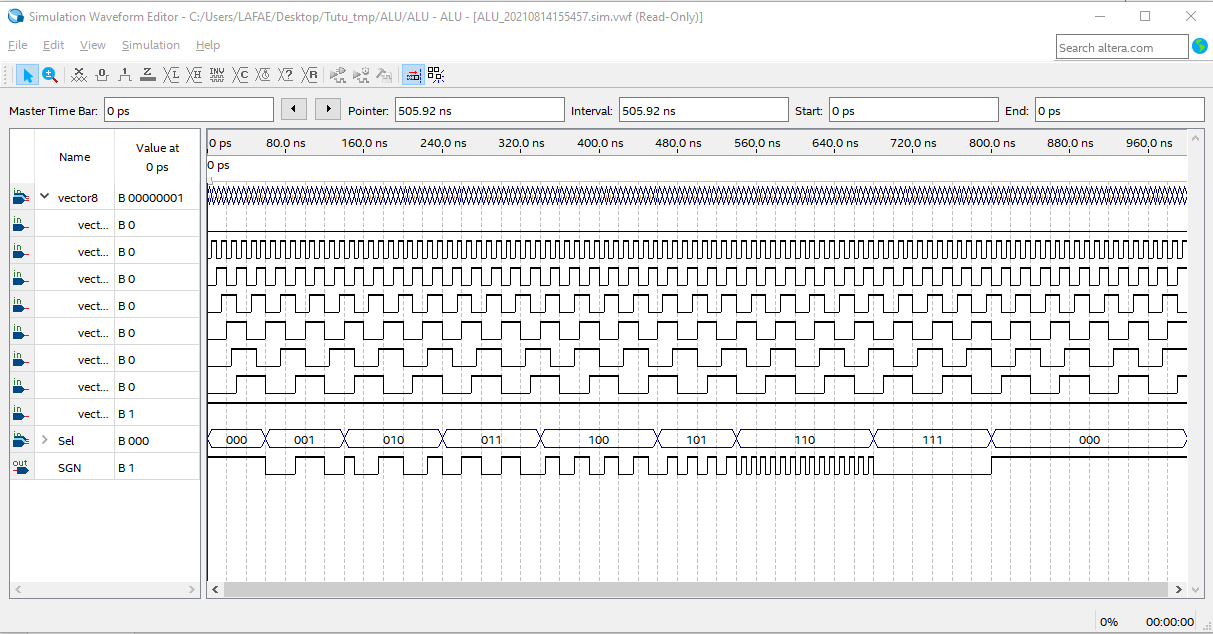
\includegraphics[width=\textwidth]{img/teste_mux.png}

\textbf{Teste contador}
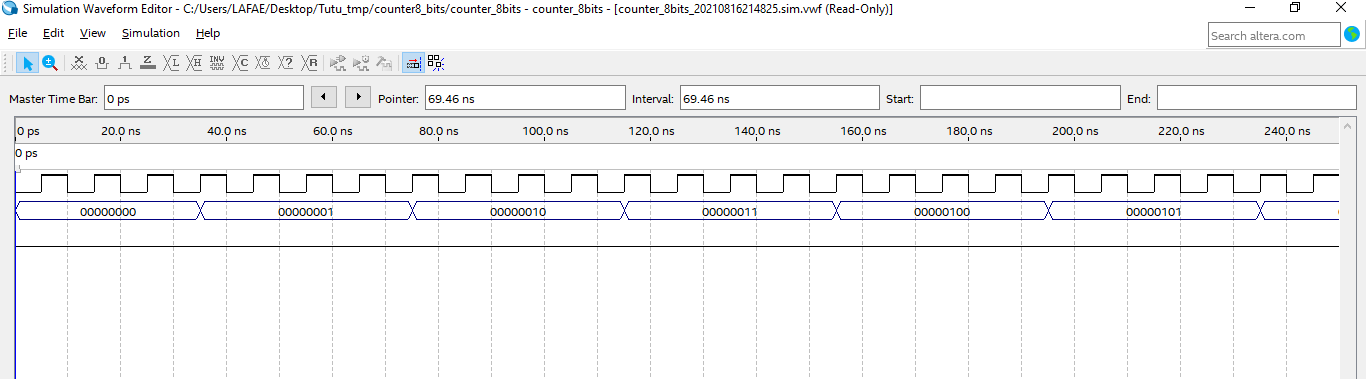
\includegraphics[width=\textwidth]{img/teste_contador.png}

\textbf{Teste ALU com contador}
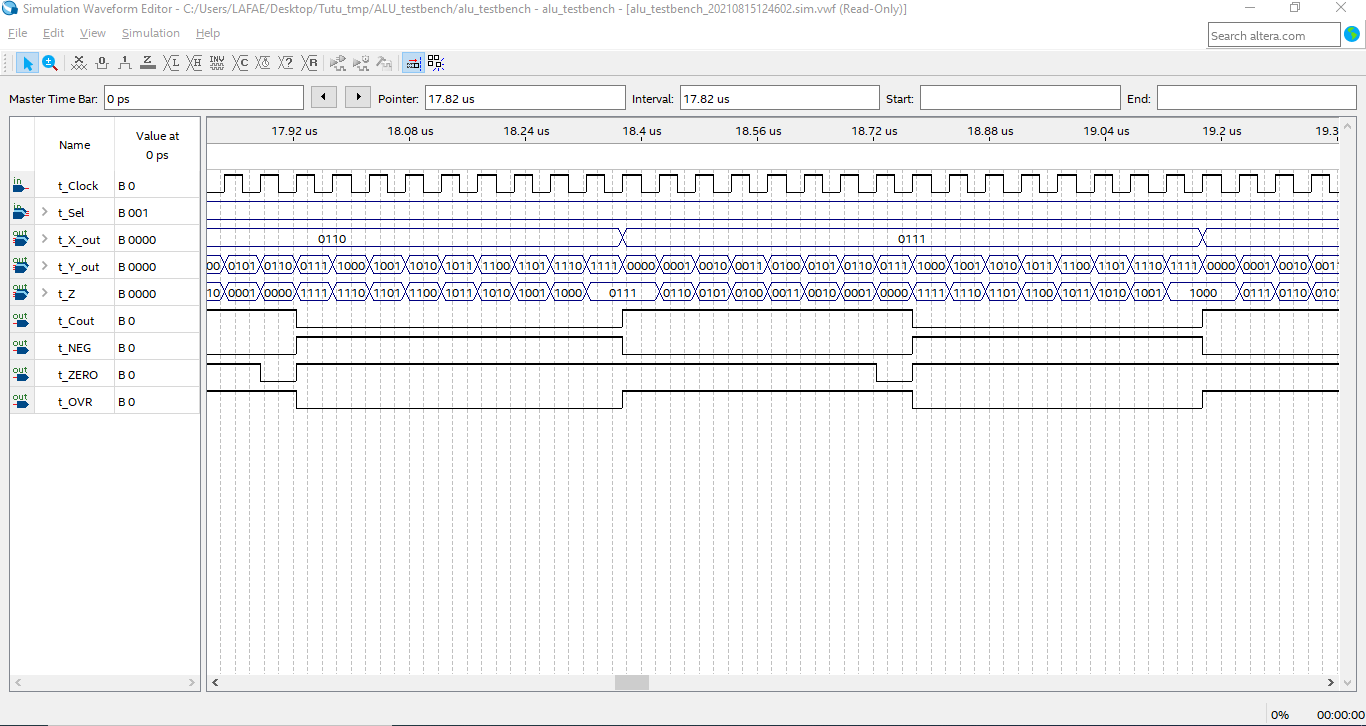
\includegraphics[width=\textwidth]{img/teste_alu_com_contador.png}
\end{center}

\section{Referências bibliográficas}


\section{Conclusão}

\section{Snapshots do funcionamento no LABSLAND}




\begin{center}

\textbf{Força zero}
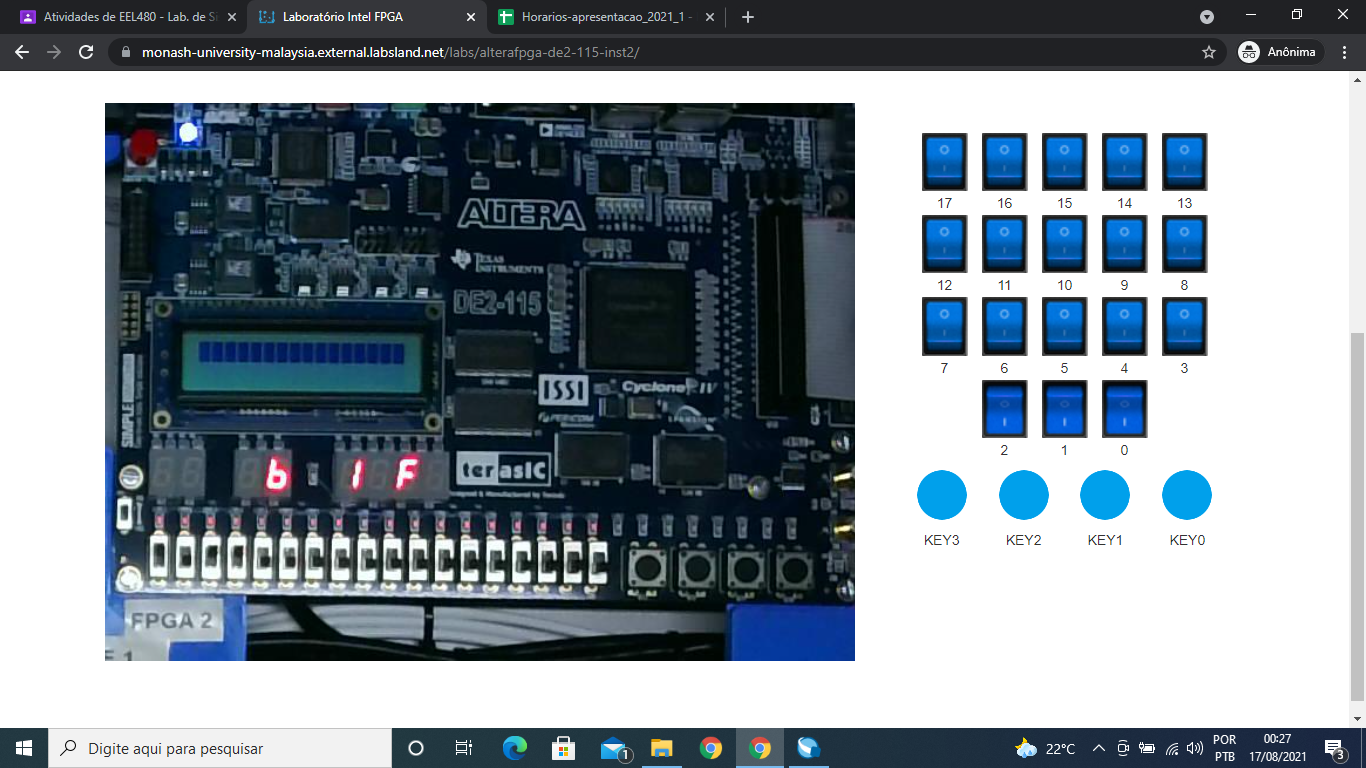
\includegraphics[width=\textwidth]{img/labsland_forca_1.png}

\textbf{Força um}
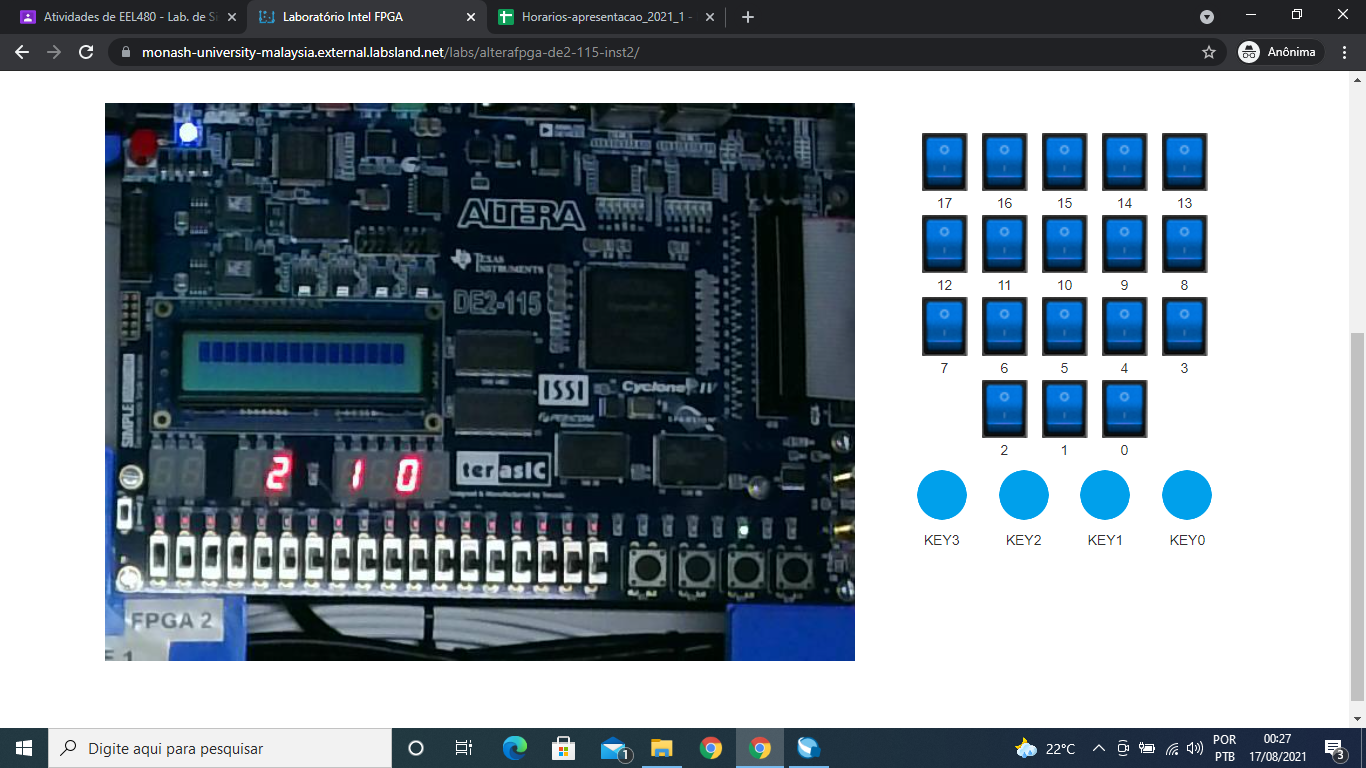
\includegraphics[width=\textwidth]{img/labsland_forca_zero.png}

\textbf{Soma: 5 + 2 = 7}
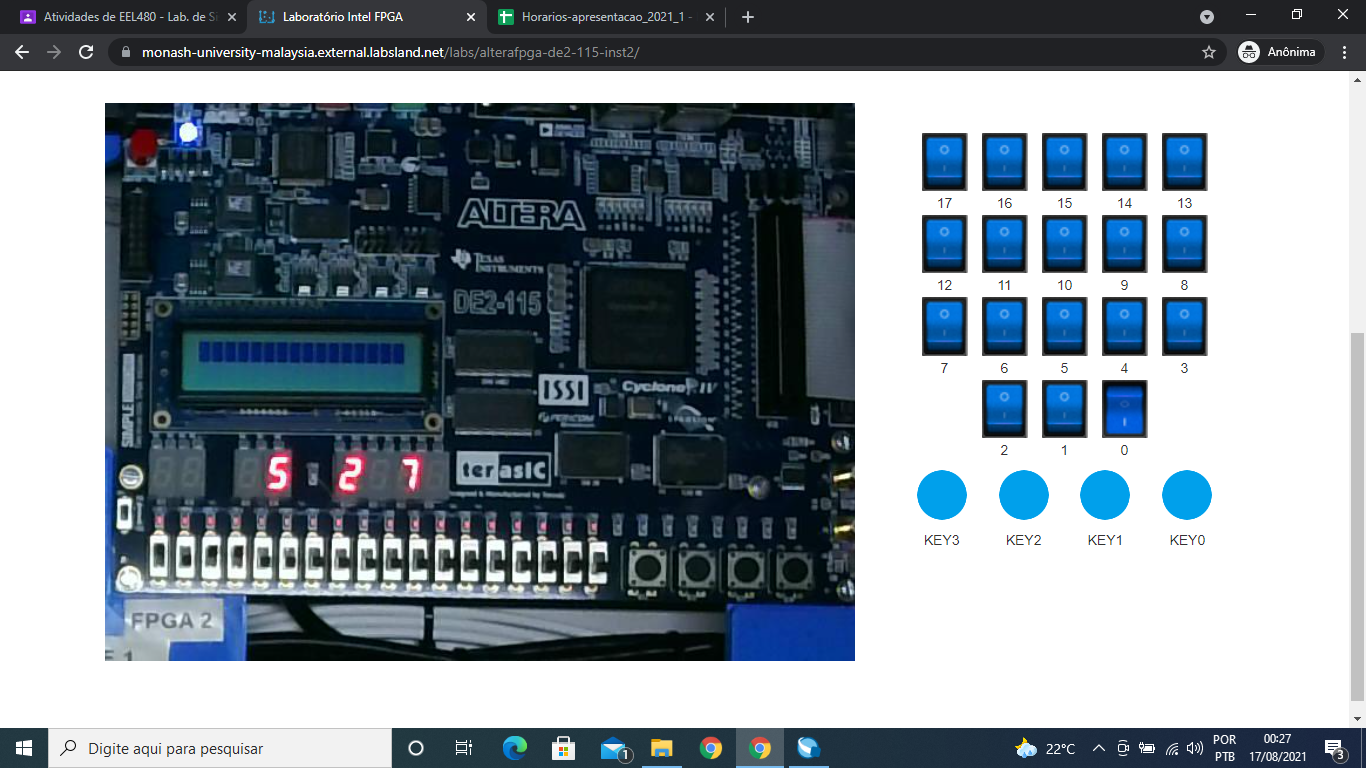
\includegraphics[width=\textwidth]{img/labsland_soma.png}

\textbf{Subtração: 1 - 4 = d (-3)} | Note a flag de negativo acessa (4 led
    partindo da direita para a esquerda)
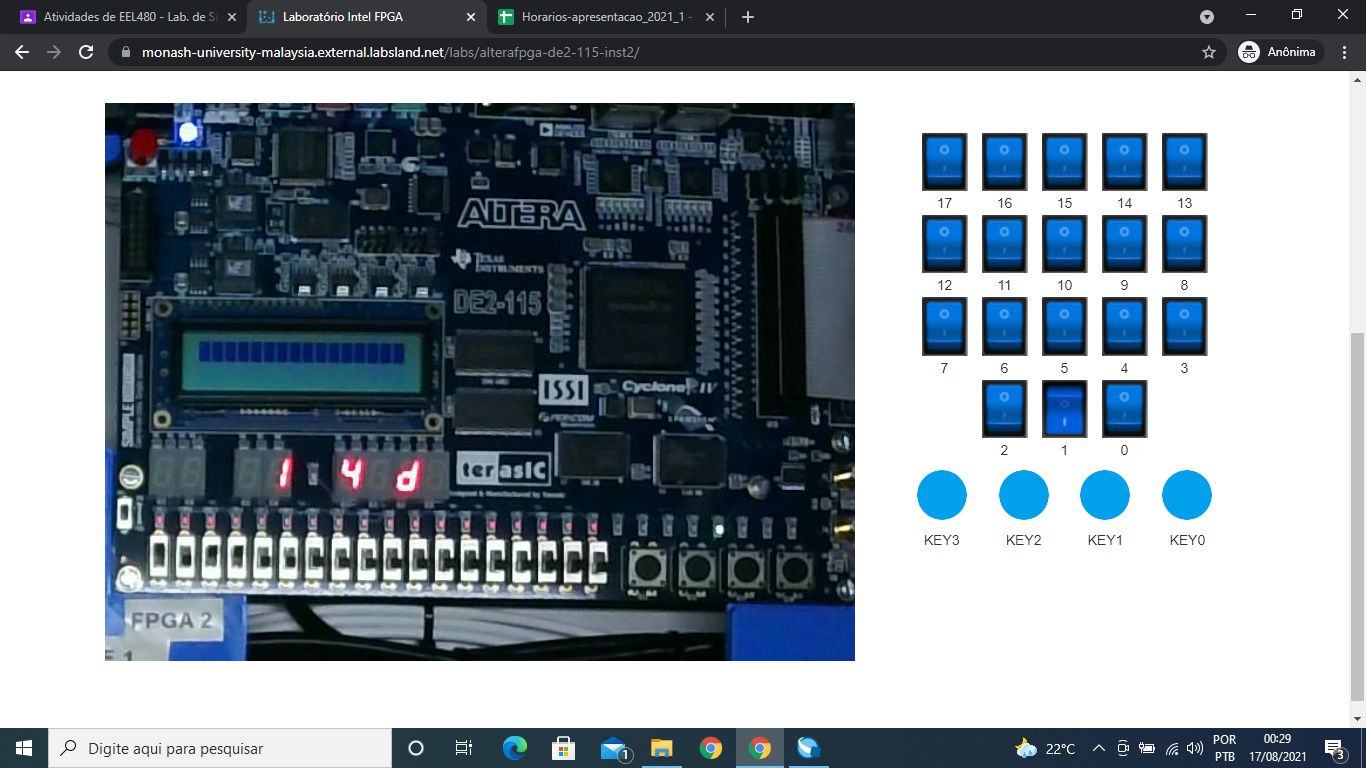
\includegraphics[width=\textwidth]{img/labsland_subtracao.png}
\end{center}

\section{Referências bibliográficas}

\end{document}
